% ===============================================================================
\section{\ij and \fiji plugin}
\wingj is released as a Java plugin for \ij (\ijWebsite), a public domain, Java-based image processing program developed at the National Institutes of Health \autocite{schneider2012nih}. If you have \ij installed on your computer, you can download the \wingj \ij plugin from the project website (\wingjShortUrl). Note that the online version of \wingj can be launched directly from a web browser. \wingj is also supported by the \ij distribution \fiji (\fijiWebsite).

% ===============================================================================
\section{Launching WingJ from any web browser}\label{sec:launch_wingj}
\wingj is distributed through the Java Web Start technology developed by Sun. This allows any computer on which Java Web Start is installed to run \wingj, independently of the operating system used. \wingj requires Java version 1.6 or later. You can test your installation on \testJavaWebsite.\\

Launching \wingj is as simple as one click. First visit our website (\wingjShortUrl) from where you will be able to run \wingj by clicking on the link \emph{Launch WingJ} present on the right side of the website. If it doesn't work, make sure that you have Java installed using the above Java test link. Java Web Start will ask whether you trust the \textit{Certificate} before downloading the application (\figref{fig:download_wingj}). A few browsers such as \chrome do not start automatically Java Web Start applications. Instead, they will download a JNLP file. In that case, locate where the JNLP file has been saved and execute it to start \wingj.\\

\begin{figure}[!h]
\centering
% \includegraphics[scale=1.5]{Logo.pdf}
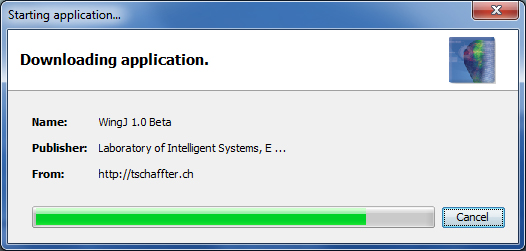
\includegraphics[scale=0.5]{images/download_wingj.jpg}
\caption{\textbf{\wingj uses the Java Web Start technology.} Click on the button \textit{Launch \wingj} from the project website (\wingjShortUrl) to start downloading the application. Java Web Start saves all the components needed to run \wingj in the Java cache, which enable to run \wingj even when no internet connection is available. Otherwise, Java Web Start automatically checks for updates each time \wingj is launched.}
\label{fig:download_wingj}
\end{figure}

% \begin{figure}[!h]
% \centering
% % \includegraphics[scale=1.5]{Logo.pdf}
% 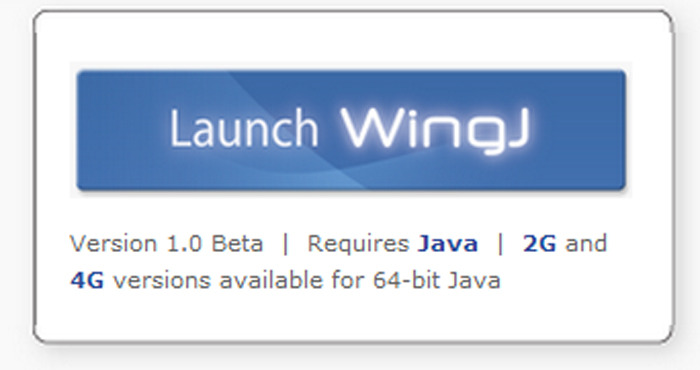
\includegraphics[scale=0.324]{images/launch_wingj.jpg}
% \caption{Click on \textit{Launch \wingj} from the project website (\wingjWebsite) to start the application. Click on \textit{2G} or \textit{4G} to allow \wingj to use more memory (requires 64-bit Java and enough physical memory to be installed).}
% \label{fig:launch_wingj}
% \end{figure}

At the end of the installation, you may be asked whether you want to install a shortcut on your Desktop.\footnote{The shortcut creation may silently fail on Mac OS X.} On Windows, a shortcut will also be placed in the \textit{Start} menu. The interface of \wingj should then appear shortly.\\

According to its default settings, Java Web Start saves all the components needed to run \wingj in the cache. This will significantly reduce the loading time compared to the first time that you launched the application. It also makes it possible to run \wingj \textit{offline}, i.e. without internet connection. If you do have an internet connection, Java Web Start will automatically check for \wingj updates.

% ===============================================================================
\section{32-bit and 64-bit versions}\label{sec:32and64-bits}
\wingj can take as input one to four stacks of confocal images, which may require large amount of memory. As an example, one stack of 38 images (1024x1024 \px) can take more than 150 \MB. The default version of \wingj doesn't set any memory requirements to allow any computer to run \wingj. Indeed, Java Web Start fails to launch an application if the specified memory requirements are not fulfilled. The drawback is that \wingj can then use only up to 250 \MB of memory (depending on the settings of your Java virtual machine). Note that this may be enough depending on the number and resolution of your images.\\

Because memory requirements have to be set before launching a Java Web Start application, we provide additional links to launch \wingj with 1 \GB, 2 \GB, and 4 \GB of memory (\wingjShortUrl). There are several requirements your machine should satisfy to run the memory-extended versions of \wingj.\\

First, enough physical memory should be installed on your machine. Note that more than 2 \GB of physical memory should be installed to run the 2 \GB version of \wingj because your operating system and additional softwares running already use part of the total amount of available memory. Most importantly, a 64-bit version of Java must be installed on your computer to run the 1 \GB, 2 \GB, and 4 \GB versions. The architecture of your operating system (OS) must also be 64-bit in order to install a 64-bit version of Java. For example, you won't be able to run the memory-extended versions of \wingj if you have a 32-bit installation of Java, even if you have 4 \GB of physical memory installed on your machine. Note that a 64-bit version of Java can be installed in complement to a 32-bit version and that the Java version effectively used can be changed at any time (by editing the system variables). Please contact your system administrator and/or refer to the Support page (\wingjShortUrl) if you have troubles with the above requirements.\\

\textbf{Tip}: There is a method to run \wingj with custom memory requirements. Download the default, 1 \GB, 2 \GB or 4 \GB \wingj JNLP file (\textit{Right click} on the link $>$ \textit{Save As}) and open this file with a text editor. Locate the parameter \textit{-Xmx}, which is used to set the maximum amount of memory \wingj can use. For example, using \textit{-Xmx2000m} allows \wingj to use up to 2 \GB of memory. Then save and execute the JNLP file. To check that the new parameter value is effective, click on \textit{ImageJ toolbar $>$ Help $>$ About ImageJ...} (\figref{fig:ij_memory}).\\

\begin{figure}[!h]
\centering
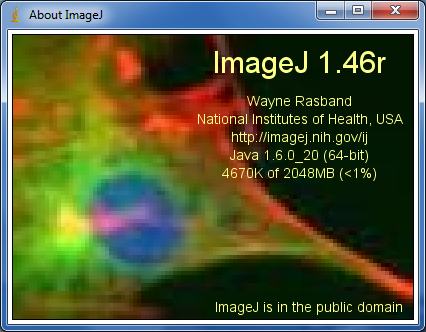
\includegraphics[scale=0.5]{images/ij_memory_2.jpg}
\caption{\textbf{Get the amount of memory that \wingj can use.} Click on \textit{ImageJ toolbar $>$ Help $>$ About ImageJ...} to know how much memory \wingj can use. Here about 2 \GB of memory are available.}
\label{fig:ij_memory}
\end{figure}

% ===============================================================================
\section{Graphical user interface}
At start up, the following graphical components are displayed as shown in \figureref{fig:wingj_interface}.

\begin{itemize}
 \item \textbf{\ij toolbar}. This toolbar includes many tools to manipulate images.
 \item \textbf{\wingj interface}. The main graphical user interface (GUI) of \wingj.
 \item \textbf{Log window}. This window gives detailed information about the running process.
\end{itemize}

\begin{figure}[!h]
\centering
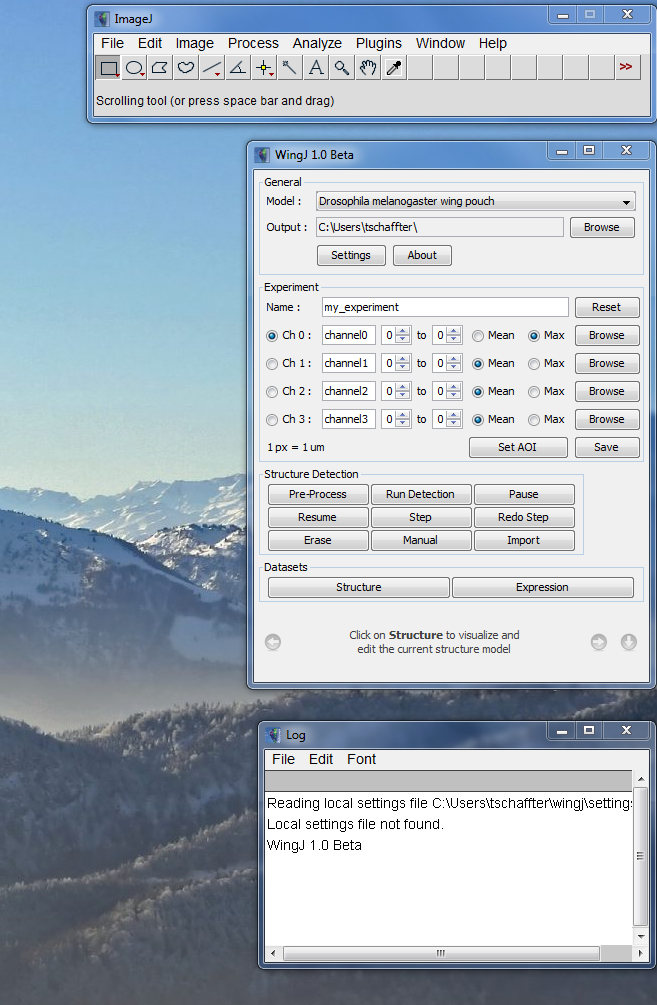
\includegraphics[scale=0.5]{images/wingj_interface_crop4.jpg}
\caption{\textbf{Graphical user interface of \wingj.} At startup, three windows are displayed: 1) the main interface of \wingj enables the detection and modelling of the morphology or biological systems, as well as the quantification of gene and protein expression, 2) the \textit{\ij toolbar} that provides tools to manipulate images, and 3) the \textit{Log window} for detailed information about the running processes.}
\label{fig:wingj_interface}
\end{figure}


% \begin{figure}[h!]
% \centering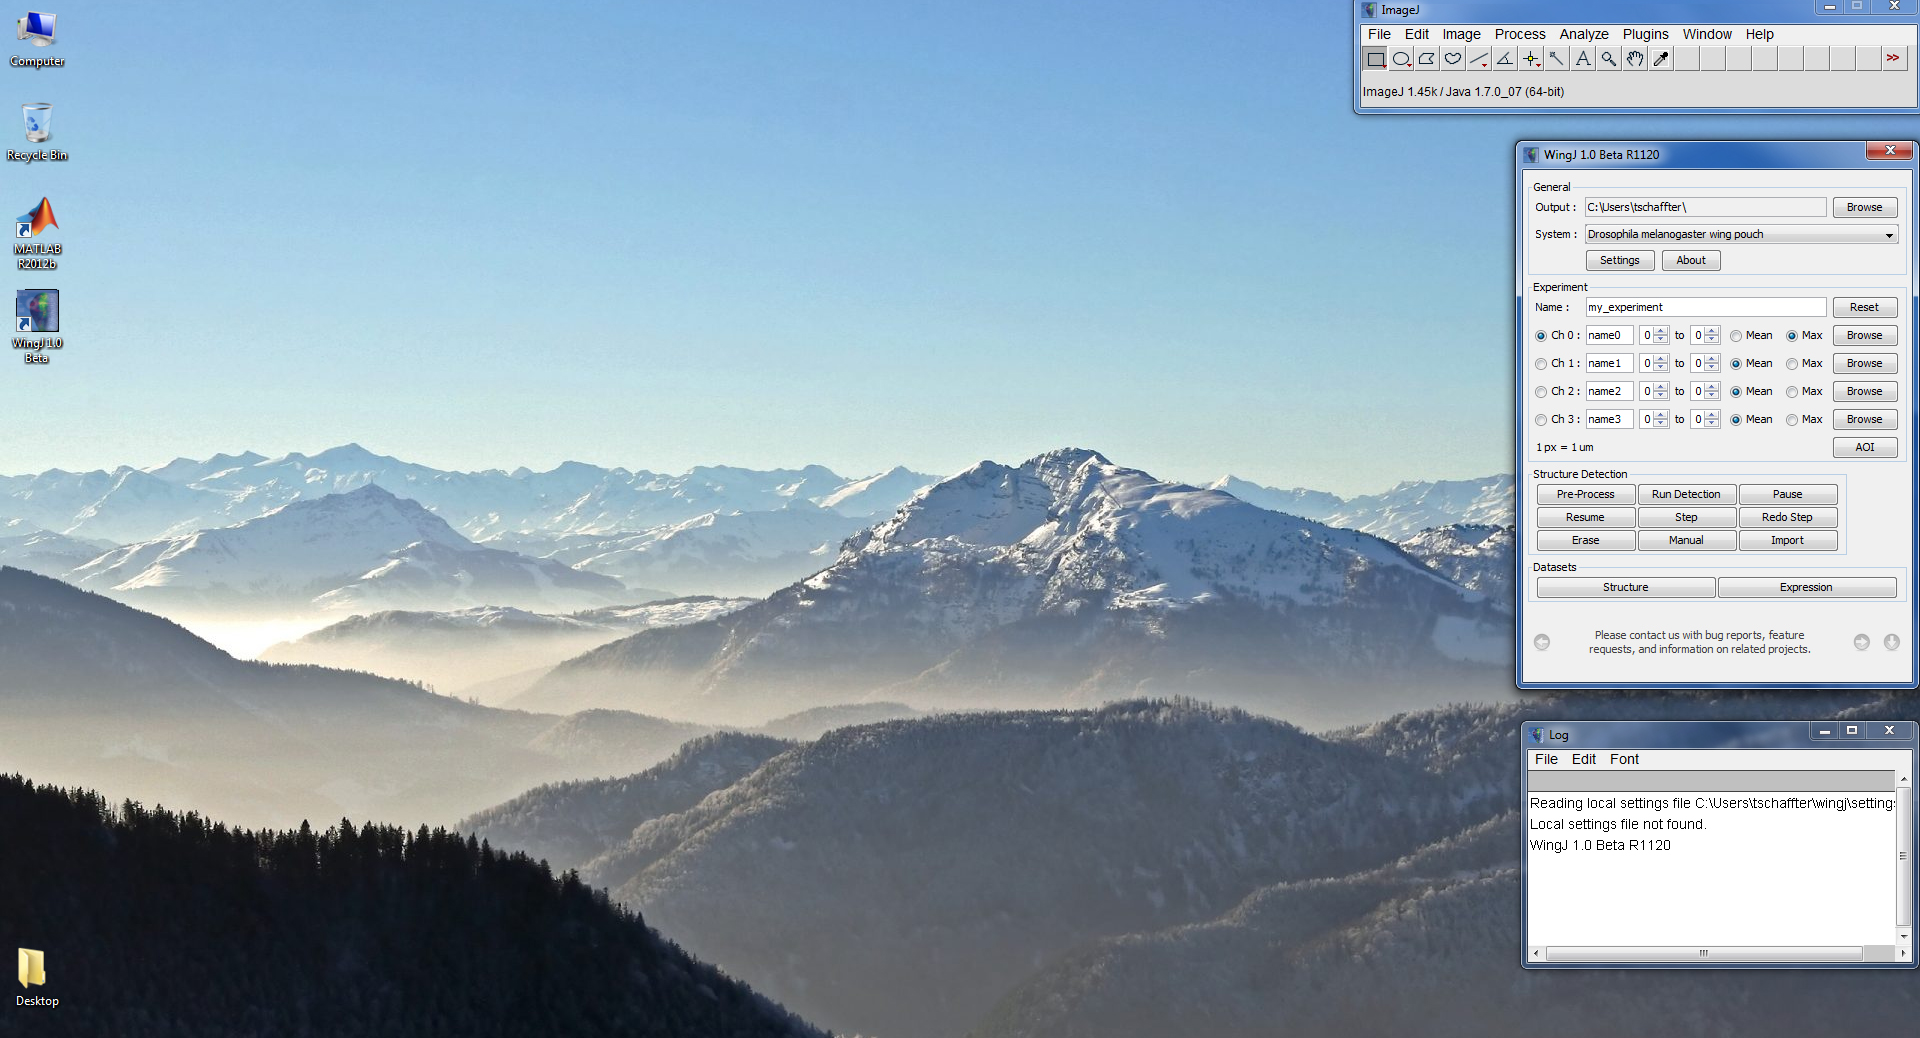
\includegraphics[width=12cm]{figures/wingj_interface}
% \caption{Interface of WingJ at startup, including the ImageJ bar and the log window.}
% \end{figure}

\textbf{Tip}: If you close the interface of \wingj, you can bring it back via \textit{ImageJ toolbar $>$ Plugins $>$ WingJ}. Close the \ij toolbar to exit \wingj.\\

\textbf{Tip}: Hold your mouse cursor over an element of the interface to display a short description (called \emph{tooltip}).


% \section{Modes}
% 
% Before commenting each element of the interface, it is important to say that WingJ can be used in two different mode. There is not that much to say about the \textit{Normal} mode which allows the user to load one by one the image stacks before running the structure detection method. In general, the \textit{Normal} mode is well suited for testing WingJ or analyzing a couple of wings. The \textit{Batch} mode has been implemented to speed up the analysis of multiple wings by automating the loading of the image stacks as well as offering a method to export all the structure and expression datasets at the same time. More information on how to run the \textit{Batch} mode are given in Section XXX.

% ===============================================================================
\section{Selecting output directory}
The \textit{output directory} tells \wingj where output files should be saved. Click on \textit{Browse} to select the output directory. When exporting datasets to files, a \textit{Save} dialog will appear and suggest you to save the files to the selected output directory. This is only a suggestion and files can actually be exported at a different location (even on network location).

% ===============================================================================
\section{Selecting active system}\label{sec:biological_system}
\wingj can be used to generate structure models for the following biological systems in an unsupervised or weakly-supervised way. The active system can be selected from a drop-down list displayed in the top part of the main interface of \wingj.

\begin{itemize}
 \item \textbf{\droso wing pouch} \autocite{schaffter2013}. Detects the structure of the wing pouch from confocal fluorescence images where the expression of Wg-Ptc is labelled using antibodies. The structure model describes the outer border (or contour) of the wing pouch (delimited by Wg), the dorsal/ventral (D/V) compartment boundary (delimited by Wg), and the anterior/posterior (A/P) compartment boundary (delimited by Ptc).
% The orientation of the model (A/P and D/V directions) is inferred from prior knowledge about the geometry of the identified structure.
 \item \textbf{\droso embryo} \autocite{schaffter2013}. Detects the structure of the embryo from the expression of any protein that allows to clearly distinct the embryo from a black background (e.g. \textit{eve} protein). The axes of the ellipse-like shape identified as the contour of the embryo are then used to define the A/P and D/V compartment boundaries.
\end{itemize}

This list will be updated as soon as additional models will be made available in \wingj. Please refer to the \wingjDeveloperGuide for instruction to developed structure detection methods for additional organ or body system.\\

\textbf{Tip}: Hold your mouse cursor over the name of the selected system to display useful information (tooltip).

% ===============================================================================
\section{Importing and exporting settings}
The graphical interface allows the user to access and modify the important settings used by \wingj. Advanced parameters are available by clicking on the button \textit{Settings}. The text area contains all the settings available in text format and modifying them should be straight forward. Please read carefully the description of each parameter. Click on \textit{Save and Close} to apply the modifications and go back to the main interface. Click on \textit{Reload} to load again the last settings file opened (the current settings will be lost if they have not be previously saved to file). To export the current settings to file, click on \textit{Export}. Click on \textit{Load} to select and load an existing settings file.\\

\textbf{Tip}: \wingj checks at startup if the file \textit{USER\_HOME/wingj/settings.txt} exists where \textit{USER\_HOME} is the path to your home directory (e.g. C:\textbackslash Users\textbackslash tschaffter\textbackslash on Windows 7 or /home/tschaffter/ on Linux). Initially, the folder \textit{wingj} doesn't exist and you would have to create it if you want to use this feature. Then modify the default settings of \wingj using the graphical interface and save them to the file \textit{USER\_HOME/wingj/ settings.txt}.

% ===============================================================================
\section{Opening stacks of confocal images} \label{sec:open_images}
\wingj takes as input stacks of confocal images or a single image (e.g. maximum or average intensity projections) to generate a parametric model of the morphology or structure of an organ system (e.g. \droso wing pouch) or body system (e.g. \droso embryo). For both wing pouch and embryo systems, the structure detection only requires one stack of images. Additional system models implemented in \wingj may have different requirements. \wingj supports up to four image stacks or image channels. Typically, one would be used as input for the structure detection method (\sectionref{chap:structure}) and the others for the quantification of gene and protein expression (\sectionref{chap:expression}).\\

Click on the button \textit{Browse} associated to an image channel to open a single image or a stack of confocal images, for instance in TIFF format. The name of the images should respect the format \textit{prefix\_Z\_C\_suffix.tif} where:

\begin{itemize}
 \item \textbf{prefix}. Is any string without white spaces ' '.
 \item \textbf{Z}. Takes the values ``z00'', ``z01'', ..., ``zN'' where N is the total number of image slices in the z-stack.
 \item \textbf{C}. Takes the values ``ch00'', ``ch01'', ``ch02''and ``ch03'' depending on which channel a given image belongs to.
 \item \textbf{suffix}. Is any string without white spaces ' '.
\end{itemize}

After having select the folder a folder containing images, a dialog named \textit{Sequence Options} appears (\figref{fig:wingj_import_stack}).\\

\begin{figure}[!h]
\centering
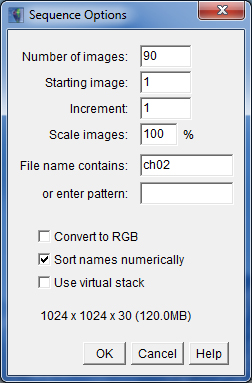
\includegraphics[scale=0.7]{images/wingj_import_stack.jpg}
\caption{\textbf{Selection of the input images for structure detection and expression quantification.} Click on the button \textit{Browse} associated to an image channel to select a folder containing images. Then, the above dialog will appear for selecting which images to open from the selected folder. Set the field \textit{File name contains} to select specific images based on their filename. Here we set it to ``ch02'' to import only the images that contains the substring ``ch02'' in their filename.}
\label{fig:wingj_import_stack}
\end{figure}

The total number of images detected in the selected folder is given by the field \textit{Number of images}. The field \textit{File name contains} allows to import only the images that belong to a given channel. By entering ``ch02'', for example, only the images whose filename contains the substring ``ch02'' will be selected and then imported. The last line of the dialog summarizes the resolution and the number of the images selected, and the amount of memory it will require to load them.\\

\textit{1024 x 1024 x 38 (152.0MB)}\\

Here the selection includes 38 images with a resolution of 1024 x 1024 pixels (\px). The image stack is taking 152 \MB of memory once loaded. Note that all the images must have the same dimensions. Click on \textit{Ok} to validate and load the selected images.\\

A window then appears to show the content of the image stack. Hold your mouse cursor over the image window and use the \emph{mouse wheel} to navigate through the stack of images. Information about the images is available in the top part of the window, including the dimensions of the images in \mum. The relation between \px and \mum is shown on the main interface of \wingj. Note that the coefficient or \emph{scale} for converting pixels to meaningful physical units (e.g. \mum) is extracted automatically by \wingj from the meta-information included in the input image files. If this is not the case, the parameters \textit{unit} and \textit{scale} can be set in the settings.\\

\textbf{Tip}: To import a single image, click on \textit{Browse}, select the folder containing the image and enter in the field \textit{File name contains} a string that uniquely identifies the image to open.\\

\textbf{Tip}: Click on \textit{Save} to export to file information about image stacks currently opened, minimum and maximum slice indexes, and projection methods selected. The next time you will click on one of the \textit{Browse} buttons and select a directory containing images, images stacks will automatically be imported in \wingj along with the additional information saved (names of the channels, minimum and maximum slice indexes, etc.). Moreover, clicking on the \emph{Save} button saves the projections of the image stacks opened to the selected output directory.\\

\textbf{Tip}: We invite you to download the \wingjBenchmarkImages to play with the different tools available in \wingj.